
% TODO: https://en.wikipedia.org/wiki/Triangle

\subsection{Cechy przystawania}
Cechy przystawania
\loremipsum
Hartshorne s. 99
% do wyrzucenia? to jest w intro

\index{pons asinorum|(}
\subsection{Pons asinorum}
%

,,\emph{Pons asinorum}'', czyli most osłów, to tradycyjna nazwa twierdzenia (I.5), że kąty przy podstawie trójkąta równoramiennego są równe.
Ci, którzy nie są w stanie samodzielnie przeprowadzić jego dedukcyjnego dowodu opartego na własnościach trójkątów przystających, nie mogą przekroczyć mostu i studiować dalej geometrii.
Bardziej przyziemnie Coxeter \cite[s. 22-24]{coxeter_1967} zauważa, że rysunek wykonany przez Euklidesa przypomni most.
Wśród konsekwencji wymienia wyniki z~Elementów: (III.3), (III.20), (III.21), (III.22), (III.32), (VI.2), (VI.4), a potem (III.35), (III.36), (VI.19), co prowadzi do dowodu twierdzenia Pitagorasa, czyli (I.47). % TODO: sprawdzić, czy numeracja moja i Coxetera jest taka sama.
\index{twierdzenie!Pitagorasa}%

\begin{figure}[H] \centering
\begin{comment}
\begin{tikzpicture}[scale=.5]
    \tkzDefPoint(90:-1){A}
    \tkzDefPoint(-55:5){C}
    \tkzDefPoint(235:5){B}
    \tkzDefPoint(-90:8){X}

    \tkzLabelPoint[above](A){$A$}
    \tkzLabelPoint[left](B){$B$}
    \tkzLabelPoint[right](C){$C$}
    \tkzInterLC(A,B)(A,X) \tkzGetPoints{XX}{D} % line and circle
    \tkzLabelPoint[left](D){$D$}
    \tkzDefLine[parallel=through D](B,C) \tkzGetPoint{XXX}
    \tkzInterLL(D,XXX)(A,C) \tkzGetPoint{E} % line and circle
    \tkzLabelPoint[right](E){$E$}
    
    \tkzMarkSegments[mark=|](A,B A,C)
    \tkzMarkSegments[mark=||](B,D C,E)
    \tkzDrawLines[add= 0 and 0, line width=0.2mm](B,E C,D)
    \tkzDrawLines[add= 0 and 0.5, line width=0.2mm](B,D C,E)
    \tkzDrawPolygon[line width=0.5mm](A,B,C)
    \tkzDrawPoints[size=4,color=black,fill=black!50](A,B,C,D,E)
\end{tikzpicture}
\end{comment}
    \caption{most osłów}
\end{figure}

Pierwsze dowody tego faktu podadzą jeszcze Euklides, komentujący jego prace Proklos, a także (dużo krócej\footnote{Pappus zauważa, że trójkąt $\triangle ABC$ przystaje do siebie $\triangle ACB$, więc stosowne kąty przy podstawie też są przystajace.}) Pappus z Aleksandrii.
\index[persons]{Proklos zwany Diadochem}%
\index[persons]{Pappus z Aleksandrii}%
Przyszłość przyniesie jeszcze jedno uzasadnienie, zaczynające się od wykreślenia dwusiecznej z kąta przy wierzchołku.
\index{dwusieczna}%
Euklides nie zrobi tego przede wszystkim ze względu na kolejność wykładanego materiału: dwusieczna pojawi się cztery tezy później, a nie można korzystać z wyników, których prawdziwości dopiero się pokaże.

O pons asinorum nie wspomina żaden szkolny podręcznik geometrii \texttt{:(}
Pojawia się u Bogdańskiej, Neugebauera \cite[s. 9]{neugebauer_2018}.

% PRZECZYTANO: https://en.wikipedia.org/wiki/Pons_asinorum

%
\index{pons asinorum|)}
\index{most osłów|see{pons asinorum}}

%

Zajmiemy się teraz (I.20).

\begin{proposition}[nierówność trójkąta]
\index{nierówność!trójkąta}%
	Niech $ABC$ będzie trojkątem.
	Wtedy suma odcinków $AB$ i $BC$ jest dłuższa niż $AC$.
\end{proposition}
% PRZECZYTANO: https://en.wikipedia.org/wiki/Triangle_inequality

\begin{proof}
	Wynika to ze wzoru Herona (fakt \ref{prp_heron}) i tego, że pole trójkąta jest nieujemne.
\end{proof}

\begin{corollary}
	Niech $a \ge b \ge c$ będą bokami trójkąta.
	Wtedy
	% \begin{equation}
	% 	1 < \frac{a + c}{b} < 3 
	% \end{equation}
	% oraz
	\begin{equation}
		1 \le \min \left(\frac ab, \frac bc\right) \le \phi = \frac {1 + \sqrt 5}{2}.
		% American Mathematical Monthly, pp. 49-50, 1954. 
	\end{equation}
\end{corollary}

Nierówność trójkąta nie jest wnioskiem z aksjomatów I1-I3, B1-B4, C1-C3, ponieważ nie zachodzi w następującym modelu (ukradniętym Hartshorne'owi \cite[s. 90]{hartshorne2000}):

\begin{example}
	Rozpatrujemy zbiór $\mathbb R^2$ jako płaszczyznę ze standardowymi punktami oraz prostymi, ale niestandardową metryką
	\begin{equation}
		d((x_1, y_1), (x_2, y_2)) = \begin{cases}
			\sqrt{(x_1-x_2)^2 + (y_1-y_2)^2} & \text{jeśli } x_1 = x_2 \vee y_1 = y_2, \\
			2 \sqrt{(x_1-x_2)^2 + (y_1-y_2)^2} & \text{w przeciwnym wypadku}
		\end{cases}.
	\end{equation}
	Wtedy nierówność trójkąta nie zachodzi.
\end{example}

% section{Problemy Fagnano i Fermata}
% https://en.wikipedia.org/wiki/Fagnano's_problem

\begin{problem}[zadanie Fagnano]
	Dany jest trójkąt ostrokątny $ABC$.
	Wpisać w niego trójkąt $UVW$ o możliwie najmniejszym obwodzie.
\index{zadanie!Fermata}%
\end{problem}

Coxeter \cite[s. 36, 37]{coxeter_1967} pokaże tak jak Fejer, że rozwiązaniem zadania jest trójkąt spodkowy (zwany ortycznym).
Audin \cite[s. 101]{audin_2003} podaje ten fakt w formie ćwiczenia. % todo: fagnano czy gemrat?

\begin{problem}[zadanie Fermata]
	\label{punkt_fermata}
	Dany jest trójkąt ostrokątny $ABC$.
	Znaleźć punkt $F$ taki, by suma $|FA| + |FB| + |FC|$ była możliwie najmniejsza.
\index{zadanie!Fermata}%
\end{problem}

\todofoot{Zadanie Fermata -- Neugebauer, s. 117.}

Powyższe zadanie rozwiąże Evangelista Torricelli (dlatego też punkt $F$ nazywa się czasem punktem Torricellego; robi tak Guzicki \cite[s. 224-228]{guzicki_2021}), który dostanie je w formie wyzwania od Fermata.
\index[persons]{Torricelli, Evangelista}%.
Rozwiązanie opublikuje student Torricelliego, Vincenzo Viviani, w 1659 roku.
\index[persons]{Viviani, Vincenzo}
% TODO: Johnson, R. A. Modern Geometry: An Elementary Treatise on the Geometry of the Triangle and the Circle. Boston, MA: Houghton Mifflin, pp. 221-222, 1929.
Coxeter \cite[s. 37]{coxeter_1967} przytoczy rozwiązanie Hofmanna\todofoot{J E Hoffman, Elementare Losung einer Mimimumsaufgabe 1929}
\index{zadanie!Fagnano}

%

\index{twierdzenie!Pitagorasa|(}
\subsection{Twierdzenie Pitagorasa}
%

Najważniejszym twierdzeniem dotyczącym trójkątów prostokątnych jest twierdzenie Pitagorasa oraz twierdzenie do niego odwrotne.
Piszą o~nim Guzicki \cite[s. 160]{guzicki_2021}.

% PRZECZYTANO: https://en.wikipedia.org/wiki/Pythagorean_theorem

\begin{theorem}[Pitagorasa]
\label{theorem_pythagorean}%
    Niech $ABC$ będzie trójkątem prostokątnym, w~którym kąt przy wierzchołku $C$ jest prosty.
    \begin{center}
\begin{comment}
        \begin{tikzpicture}[scale=.4]
        %\tkzInit[xmin=-0.5,xmax=6.5, ymin=-0.5,ymax=4.5]
        % \tkzClip
        \tkzDefPoint(105:3){A}
        \tkzDefPoint(285:3){B}
        \tkzDefPoint(35:3){C}
        \tkzDefPoint(35:4.75){CC}
        \tkzMarkRightAngle[size=0.5](A,C,B)

        \tkzLabelPoint[above left](A){$A$}
        \tkzLabelPoint[below](B){$B$}
        \tkzLabelPoint[below left](CC){$C$}
        \tkzDefSquare(B,A)
        \tkzDrawPolygon[fill=black!50](B,A,tkzFirstPointResult, tkzSecondPointResult)
        \tkzDefSquare(C,B)
        \tkzDrawPolygon[fill=black!25](C,B,tkzFirstPointResult, tkzSecondPointResult)
        \tkzDefSquare(A,C)
        \tkzDrawPolygon[fill=black!25](A,C,tkzFirstPointResult, tkzSecondPointResult)
        \tkzDrawPolygon[line width=0.4mm](A,B,C)
    \end{tikzpicture}
\end{comment}
    \end{center}
    Wtedy suma pól jasnych kwadratów jest równa polu ciemnego kwadratu:
    \begin{equation}
        |AC|^2 + |BC|^2 = |AB|^2.
    \end{equation}
    Odwrotnie, jeśli $ABC$ jest trójkątem takim, że $|AC|^2 + |BC|^2 = |AB|^2$, to trójkąt ten jest prostokątny, zaś kąt przy wierzchołku $C$ jest prosty.
\end{theorem}

Powyższe twierdzenie przypiszemy kiedyś Pitagorasowi z~Samos, choć nie wiemy dokładnie, kto i~kiedy odkryje je jako pierwszy.
\index[persons]{Pitagoras z Samos}%
Będzie powszechnie stosowane w~okresie Starego Babilonu (XX-XVI wiek p.n.e.), a~więc na długo przed narodzinami Pitagorasa; pojawi się też w~indyjskich i~chińskich tekstach matematycznych.
Papirus Berlin 6619 spisany ok. 1800 roku p.n.e. na terenach państwa egipskiego zawrze zadanie, którego rozwiązaniem jest trójka $(6, 8, 10)$.
\index{papirus Berlin 6619}%
Jest jeszcze babilońska tabliczka Plimpton 322, także spisana ok. 1800 roku p.n.e., gdzie pojawia się trójka
\begin{equation}
    12709^2 + 13500^2 = 18541^2,
\end{equation}
co sugeruje, że jej autor znał pewną systematyczną metodę.
\index{tabliczka Plimpton 322}%

Być może twierdzenie Pitagorasa ma więcej znanych dowodów niż jakiekolwiek inne (poza prawem wzajemności reszt kwadratowych).
Będzie ich tak bardzo bez liku, że nie wiadomo, ile dokładnie.
Niektóre opierają się na rozcięciu pewnej układanki na fragmenty, przestawieniu ich i~zbudowaniu innego kształtu.
Inne korzystają z podobieństwa trójkątów.
Dowód Euklidesa urzekł nas tak bardzo swoją pomysłowością, że będzie jedynym, jaki przedstawimy w~całej książce!
\index{zasada!Cavalieriego}

\begin{proof}
    Niech $\triangle ABC$ będzie trójkątem prostokątnym, z kątem prostym przy wierzchołku $C$.
    Na bokach $BC$, $AB$, $CA$ kreślimy kolejno kwadraty $BCDE$, $ABFG$, $ACHI$ (konstrukcja kwadratu Euklidesa korzysta z postulatu równoległości).

    \begin{center}
\begin{comment}
            \begin{tikzpicture}[scale=.4]
        %\tkzInit[xmin=-0.5,xmax=6.5, ymin=-0.5,ymax=4.5]
        % \tkzClip
        \tkzDefPoint(105:3){A}
        \tkzDefPoint(285:3){B}
        \tkzDefPoint(35:3){C}
        \tkzDefPoint(35:4.75){CC}

        \tkzLabelPoint[above left](A){$A$}
        \tkzLabelPoint[below](B){$B$}
        \tkzLabelPoint[below left](CC){$C$}
        \tkzDefSquare(B,A)
        \tkzGetPoints{G}{F}
        \tkzLabelPoint[below](F){$F$}
        \tkzLabelPoint[above](G){$G$}
        \tkzDefPointsBy[projection=onto A--B](C){K}
        \tkzDefPointsBy[projection=onto G--F](C){L}

        \tkzDrawPolygon[line width=0.3mm, fill=blue!10](A,K,L,G)
        \tkzDrawPolygon[line width=0.3mm, fill=red!10](B,K,L,F)
        \tkzDrawPolygon[line width=0.3mm](A,B,F,G)
        \tkzLabelPoint[below left](K){$K$}
        \tkzLabelPoint[left](L){$L$}


        \tkzDefSquare(C,B)
        \tkzGetPoints{E}{D}
        \tkzDrawPolygon[line width=0.3mm,fill=red!40](C,B,E,D)
        \tkzLabelPoint[above](D){$D$}
        \tkzLabelPoint[below](E){$E$}
        \tkzDefSquare(A,C)
        \tkzGetPoints{H}{I}
        \tkzDrawPolygon[line width=0.3mm, fill=blue!40](A,C,H,I)
        \tkzLabelPoint[above right](H){$H$}
        \tkzLabelPoint[above right](I){$I$}
        \tkzDrawSegments[line width=0.2mm](C,G)
        \tkzDrawSegments[line width=0.2mm, dashed](C,K)
        \tkzDrawSegments[line width=0.2mm](I,B)
        % \tkzMarkRightAngle[size=0.5](A,C,B)
        \tkzDrawPolygon[line width=0.5mm](A,B,C)
    \end{tikzpicture}
\end{comment}
    \end{center}
    Z punktu $C$ opuszczamy wysokość na przeciwprostokątną $AB$ i przedłużamy tak, by przecięła kwadrat $ABFG$ w punktach $K$ i $L$.
    Łączymy punkty $B$ i $I$ oraz $C$ i $G$.
    Otrzymane trójkąty $\triangle BAI$ oraz $\triangle GAC$ są przystające na mocy cechy bok-kąt-bok ($AB$, $\angle BAI$, $AI$ oraz $AG$, $\angle GAC$, $AC$).
    Niebieski prostokąt $AGLK$ (odpowiednio: kwadrat $ACHI$) ma dwukrotnie większe pole niż trójkąt $\triangle GAC$ (trójkąt $\triangle BAI$).
    (To jest zamaskowana zasada Cavalieriego!).
    \index{zasada Cavalieriego}%
    Zatem prostokąt $AGLK$ i~kwadrat $ACHI$ mają równe pola.
    
    Analogicznie pokazujemy, że czerwony prostokąt $BFLK$ i kwadrat $BCDE$ mają równe pola.
    Dodajemy dwie równości stronami i otrzymujemy, że suma pól kwadratów $ACIH$ oraz $BCDE$ jest równa polu kwadratu $ABFG$.
\end{proof}

Według legendy Hippazos z Metapontu odkryje, że przekątna kwadratu (albo, według innej legendy, pięciokąta) nie jest współmierna z~jego bokiem.
Niewymierność liczb $\sqrt{2}$ (albo $(1 + \sqrt 5) /2$) zrujnuje pogląd szkoły pitagorejskiej, że świat opiera się na liczbach (co dla ówczesnych znaczyć będzie: liczb naturalnych oraz ułamków z nich zbudowanych) i doprowadzi do utopienia Hippazosa.
\index[persons]{Hippazos z Metapontu}%
\index{utopienie}%
Ale jego śmierć nie cofnie rozłamu, jaki powstanie w szkole.

(Być może w tym miejscu warto dowiedzieć się o cegle Eulera.)

\begin{corollary}
    Długość przekątnej prostokąta o bokach długości $a$ i $b$ wynosi $\sqrt{a^2 + b^2}$.
\end{corollary}

Względnie pierwsze liczby naturalne $a, b, c$ takie, że $a^2 + b^2 = c^2$ nazywamy (pierwotną) trójką pitagorejską.
\index{trójka pitagorejska}%
Każdą taką trójkę można otrzymać biorąc względnie pierwsze liczby $m, n$ różnej parzystości takie, że $m > n$ i kładąc $a = m^2 - n^2$, $b = 2 mn$, $c = m^2 + n^2$.
Najmniejszą taką trójką jest $(3, 4, 5)$; inna legenda (nie było w niej ani smoków, ani Hippazosa) głosi, że Egipcjanie używali tego trójkąta do wyznaczania kątów prostych u podstawy piramid.

\begin{proposition}
    % TODO: rysunek z Guzickiego, stron 160
    Niech $\triangle ABC$ będzie trójkątem prostokątnym, z kątem prostym przy wierzchołku $C$:
        \begin{center}
\begin{comment}
    \begin{tikzpicture}[scale=.4]
        \tkzDefPoint(200:5){A}
        \tkzDefPoint(20:5){B}
        \tkzDefPoint(90:5){C}
        \tkzDefPointsBy[projection=onto A--B](C){D}
        \tkzLabelPoint[below left](200:5){A}
        \tkzLabelPoint[below right](22:5.3){B}
        \tkzLabelPoint[above](90:5.2){C}
        
        \tkzMarkRightAngle[size=0.8](A,C,B)
        \tkzDrawPolygons[line width=0.2mm](A,B,C)
        \tkzDrawSegment[dim={$\,\,p\,\,$,-8pt,transform shape,sloped}](A,D)
        \tkzDrawSegment[dim={$\,\,q\,\,$,-8pt,transform shape,sloped}](D,B)
        \tkzDrawSegment[dim={$\,\,b\,\,$,-8pt,transform shape,sloped}](C,A)
        \tkzDrawSegment[dim={$\,\,a\,\,$,-8pt,transform shape,sloped}](B,C)
        \tkzDrawPoints[size=3,color=black,fill=black!50](A,B,C)
        \tkzDrawSegment[dim={$\,\,h\,\,$,-0pt,transform shape,sloped}](C,D)
\end{tikzpicture}
\end{comment}
    \end{center}
    Mają wtedy miejsce następujące równości:
    \begin{equation}
        h = \frac{ab}{c}, \quad
        p = \frac{b^2}{c}, \quad
        q = \frac{a^2}{c}, \quad
        h^2 = pq.
    \end{equation}
\end{proposition}

Twierdzenie Pitagorasa znajduje zastosowanie także przy wyznaczaniu niektórych miejsc geometrycznych.

\begin{proposition}
    Dane są dwa różne punkty $A$ i $B$ na płaszczyźnie oraz liczba rzeczywista $c$ taka, że $2c > |AB|^2$.
    Miejscem geometrycznym punktów $P$ o własności $|AP|^2 + |BP|^2 = c$ jest okrąg o środku w środku odcinka $AB$ i promieniu $r = \frac 1 2 \sqrt{2c - |AB|^2}$.
\end{proposition}

\begin{proposition}
    Dane są dwa różne punkty $A$ i $B$ na płaszczyźnie oraz liczba rzeczywista $c$.
    Miejscem geometrycznym punktów $P$ o własności $|AP|^2 - |BP|^2 = c$ jest prosta prostopadła do prostej $AB$.
\end{proposition}

Patrz Guzicki \cite[s. 170-173]{guzicki_2021} (Guzicki wprowadza potem osie i środki potęgowe jak w~fakcie \ref{guzicki_6_11}, a następnie twierdzenie \ref{guzicki_6_13} (Carnota)).

Spirala Teodor(os)a z Cyreny składa się z trójkątów prostokątnych stykających się ze sobą wzdłuż boków.
\index{spirala Teodorusa}%
\index[persons]{Teodor(os) z Cyreny}%
Zaczynamy od trójkąta prostokątnego równoramiennego, o bokach długości $1$, $1$, $\sqrt{2}$, by następnie kreślić jednostkowy odcinek prostopadły do końca przeciwprostokątnej, łączymy go z~początkiem i powtarzamy (Teodoros zatrzyma się na trójkącie, którego najdłuższy bok to $\sqrt{17}$, ponieważ następny naszedłby na ten, od którego zaczynaliśmy).
\begin{center}
\begin{comment}
    \begin{tikzpicture}[scale=.7]
        \tkzDefPoints{0.0000000000000000/0.0000000000000000/sqrt0,1.0000000000000000/0.0000000000000000/sqrt1,1.0000000000000002/1.0000000000000000/sqrt2,0.2928932188134524/1.7071067811865475/sqrt3,-0.6927053408400360/1.8762087599123103/sqrt4,-1.6308097207961914/1.5298560894922923/sqrt5,-2.3149821631755443/0.8005358106787454/sqrt6,-2.6417995393402450/-0.1445516998920071/sqrt7,-2.5871641322679750/-1.1430580705747615/sqrt8,-2.1830320757712630/-2.0577587215594090/sqrt9,-1.4971125019181266/-2.7854360801498297/sqrt10,-0.6162802729096475/-3.2588646221072777/sqrt11,0.3663043810988235/-3.4446801158290160/sqrt12,1.3606978771718410/-3.3389371493126440/sqrt13,2.2867524231255560/-2.9615474595774080/sqrt14,3.0782592751547995/-2.3503871670266260/sqrt15,3.6851266321570497/-1.5555840398277552/sqrt16,4.0740226421139890/-0.634302381788492/sqrt17}
        \tkzDrawPolygons[line width=0.2mm](sqrt0,sqrt1,sqrt2 sqrt0,sqrt2,sqrt3 sqrt0,sqrt3,sqrt4 sqrt0,sqrt4,sqrt5 sqrt0,sqrt5,sqrt6 sqrt0,sqrt6,sqrt7 sqrt0,sqrt7,sqrt8 sqrt0,sqrt8,sqrt9 sqrt0,sqrt9,sqrt10 sqrt0,sqrt10,sqrt11 sqrt0,sqrt11,sqrt12 sqrt0,sqrt12,sqrt13 sqrt0,sqrt13,sqrt14 sqrt0,sqrt14,sqrt15 sqrt0,sqrt15,sqrt16 sqrt0,sqrt16,sqrt17)
        \tkzMarkRightAngle[size=0.25](sqrt0,sqrt1,sqrt2)
        \tkzMarkRightAngle[size=0.25](sqrt0,sqrt2,sqrt3)
        \tkzMarkRightAngle[size=0.25](sqrt0,sqrt3,sqrt4)
        \tkzMarkRightAngle[size=0.25](sqrt0,sqrt4,sqrt5)
        \tkzMarkRightAngle[size=0.25](sqrt0,sqrt5,sqrt6)
        \tkzMarkRightAngle[size=0.25](sqrt0,sqrt6,sqrt7)
        \tkzMarkRightAngle[size=0.25](sqrt0,sqrt7,sqrt8)
        \tkzMarkRightAngle[size=0.25](sqrt0,sqrt8,sqrt9)
        \tkzMarkRightAngle[size=0.25](sqrt0,sqrt9,sqrt10)
        \tkzMarkRightAngle[size=0.25](sqrt0,sqrt10,sqrt11)
        \tkzMarkRightAngle[size=0.25](sqrt0,sqrt11,sqrt12)
        \tkzMarkRightAngle[size=0.25](sqrt0,sqrt12,sqrt13)
        \tkzMarkRightAngle[size=0.25](sqrt0,sqrt13,sqrt14)
        \tkzMarkRightAngle[size=0.25](sqrt0,sqrt14,sqrt15)
        \tkzMarkRightAngle[size=0.25](sqrt0,sqrt15,sqrt16)
        \tkzMarkRightAngle[size=0.25](sqrt0,sqrt16,sqrt17)
\end{tikzpicture}
\end{comment}
\end{center}
Niektórzy nazywają otrzymaną figurę ślimakiem pitagorejskim.
\index{ślimak pitagorejski}
\index{twierdzenie!Pitagorasa|)}

\index{wzór!Herona|(}
\subsection{Wzór Herona}
%
\subsubsection{Wzór Herona}

\index{wzór!Herona|(}
Guzicki \cite[s. 165-168]{guzicki_2021} wyprowadza wzór Herona z twierdzenia Pitagorasa.
\index{twierdzenie!Pitagorasa}
Oryginalny dowód Herona był dość skomplikowany, Guzicki \cite[s. 168-169]{guzicki_2021} wspomina o znacznie prostszym dowodzie geometrycznym, pochodzącym od Eulera.
\index[persons]{Euler, Leonhard}%
(Chociaż wynik przypisujemy obecnie Heronowi, został odkryty przez Archimedesa -- Coxeter \cite[s. 12]{coxeter_1991} odsyła do van der Waerdena \cite{MISSING_CITATION}).
% This remarkable expression, which we shall use in § 18.4, is attributed to Heron of Alexandria (about 60 a.d.), but it was really discovered by Archimedes. (See B. L. van der Waerden, Science Awakening, Oxford University Press, New York, 1961, pp. 228, 277.) 

\index{wzór!Herona|)}

% TODO: wzór Herona (Guzicki-6), Brahmagupty

%
\index{wzór!Herona|)}

\subsection{Symetralna i okrąg opisany}
Symetralna i okrąg opisany
\loremipsum

\subsection{Ortocentrum}
Ortocentrum.
\loremipsum

\subsection{Problemy Fagnano i Fermata}
Problemy Fagnano i Fermata % https://en.wikipedia.org/wiki/Fagnano's_problem
\todofoot{Coxeter, s. 20, 21}
Audin \cite[s. 101]{audin_2003} podaje ten fakt w formie ćwiczenia.

\begin{problem}[zadanie Fermata]
	Dany jest trójkąt $ABC$.
	Znaleźć punkt $F$ taki, by suma $|FA| + |FB| + |FC|$ była możliwie najmniejsza.
\index{zadanie!Fermata}%
\end{problem}

% Zadanie Fermata -- Neugebauer, s. 117.

Powyższe zadanie rozwiąże Evangelista Torricelli, który dostał je w formie wyzwania od Fermata.
\index[persons]{Torricelli, Evangelista}%
Rozwiązanie opublikował student Torricelliego, Viviani, w 1659 roku.
\index[persons]{Viviani, ???}
% TODO: Johnson, R. A. Modern Geometry: An Elementary Treatise on the Geometry of the Triangle and the Circle. Boston, MA: Houghton Mifflin, pp. 221-222, 1929.
\todofoot{Punkt Fermata (punkt Torricellego) - punkt w trójkącie, którego suma odległości od wierzchołków trójkąta jest najmniejsza z możliwych. Pierwszy raz problem konstrukcji takiego punktu został rozwiązany przez Fermata w prywatnym liście.}. %https://pl.wikipedia.org/wiki/Punkt_Fermata

\index{zadanie!Fagnano}

\subsection{Nierówności trójkątne}

\begin{proposition}[nierówność izoperymetryczna]
	Dany jest trójkąt o połowie obwodu $p$ oraz polu $S$.
	Wtedy 
	\begin{equation}
		S \le \frac{p^2}{3 \sqrt 3},
	\end{equation}
	zatem wśród trójkątów o ustalonym obwodzie największe pole ma trójkąt równoboczny.
\end{proposition}

Guzicki \cite[s. 169, 170]{guzicki_2021} wyprowadza nierówność izoperymetryczną ze wzoru Herona oraz nierówności między średnią arytmetyczną i geometryczną.
\index{wzór Herona}

% trójwymiarowy odpowiednik to hipoteza: https://math.stackexchange.com/questions/4044670/what-is-the-largest-volume-of-a-polyhedron-whose-skeleton-has-total-length-1-is

\begin{proposition}[stosunek sumy środkowych do obwodu]
	Niech... % stosunek sumy środkowych do obwodu leży między 3/4 i 1 (s. 355),
	% TODO: https://en.wikipedia.org/wiki/Isoperimetric_inequality ?
\end{proposition}

\begin{proposition}[nierówność Eulera]
	$R \ge 2r$
	% TODO: Twierdzenie Eulera: $d^2 = R^2 - 2Rr$. % Audin \cite[s. 110]{audin_2003} podaje ten fakt w formie ćwiczenia.

	% TODO: Eulera: R >= 2r https://en.wikipedia.org/wiki/Euler%27s_theorem_in_geometry
	\todofoot{formuła Eulera na odległość między środkami okręgu opisanego i wpisanego (dla trójkąta)}
\end{proposition}

\begin{proposition}[nierówność Mitrinovica]
	Niech...
\end{proposition}

\begin{proposition}[nierówność Leibniza]
	Niech...
\end{proposition}

\begin{proposition}[nierówność Weitzenbocka]
	Niech...
	% TODO: https://en.wikipedia.org/wiki/Hadwiger–Finsler_inequality => Weitzenbock
	% TODO: https://en.wikipedia.org/wiki/Pedoe%27s_inequality => Weitzenbock
\end{proposition}

Snellius-Huygens: $2 \sin x + \tan x > 3x$.

%

\label{subsection_erdos_mordell}
Erdős w 1935 roku postawi problem dowodu tej nierówności; dowód przedstawią dwa lata później Mordell i D. F. Barrow (1937), choć nie będzie on zbyt elementarny.
Później znajdzie się prostsze dowody: Kazarinoff (1957), Bankoff (1958) oraz Alsina i Nelsen (2007).
% TODO: https://en.wikipedia.org/wiki/Erdős–Mordell_inequality#CITEREFErdős1935

\begin{theorem}[nierówność Erdősa-Mordella]
    Niech $P$ będzie punktem wewnątrz trójkąta $\triangle ABC$, zaś $A_p, B_p, C_p$ spodkami punktu $P$ na boki trójkąta jak na rysunku \ref{erdos_mordell_barrowa}.
    Wtedy
    \begin{equation}
        |PA| + |PB| + |PC| \ge 2 (|PA_p| + |PB_p| + |PC_p|).
    \end{equation}
\end{theorem}


\begin{figure}[H] \centering
\begin{minipage}[b]{.45\linewidth}
\begin{center}\begin{tikzpicture}[scale=.4]
    \tkzDefPoint(0, 0){A}
    \tkzDefPoint(10, 2){B}
    \tkzDefPoint(6, 7){C}
    \tkzDefPoint(5, 3){P}
    \tkzLabelPoint[below left](A){$A$}
    \tkzLabelPoint[below right](B){$B$}
    \tkzLabelPoint[above](C){$C$}
    \tkzLabelPoint[below left](P){$P$}
    \tkzDefPointsBy[projection=onto A--B](P){Pc}
    \tkzDefPointsBy[projection=onto B--C](P){Pa}
    \tkzDefPointsBy[projection=onto C--A](P){Pb}
    \tkzLabelPoint[above right](Pa){$A_p$}
    \tkzLabelPoint[above left](Pb){$B_p$}
    \tkzLabelPoint[below](Pc){$C_p$}

    \tkzDrawSegments[line width=0.2mm,dashed](P,Pa P,Pb P,Pc)
    \tkzDrawPolygon[line width=0.3mm](A,B,C)
    \tkzMarkRightAngles[size=0.5](P,Pa,C P,Pb,A P,Pc,B)
    \tkzDrawPoints[size=3,color=black,fill=black!50](A,B,C,P,Pc,Pb,Pa)
\end{tikzpicture}\end{center}
    \subcaption{nierówność Erdősa-Mordella}
    \label{erdos_mordell_barrowa}
\end{minipage}
%
\begin{minipage}[b]{.45\linewidth}
\begin{center}\begin{tikzpicture}[scale=.4]
    \tkzDefPoint(0, 0){A}
    \tkzDefPoint(10, 2){B}
    \tkzDefPoint(6, 7){C}
    \tkzDefPoint(5, 3){P}

    \tkzDefLine[bisector](A,P,B) \tkzGetPoint{prePc}
    \tkzInterLL(P,prePc)(A,B) \tkzGetPoint{Pc}
    \tkzDefLine[bisector](B,P,C) \tkzGetPoint{prePa}
    \tkzInterLL(P,prePa)(B,C) \tkzGetPoint{Pa}
    \tkzDefLine[bisector](C,P,A) \tkzGetPoint{prePb}
    \tkzInterLL(P,prePb)(C,A) \tkzGetPoint{Pb}

    \tkzLabelPoint[below left](A){$A$}
    \tkzLabelPoint[below right](B){$B$}
    \tkzLabelPoint[above](C){$C$}
    %\tkzLabelPoint[below left](P){$P$}
    \tkzLabelPoint[above right](Pa){$A_p$}
    \tkzLabelPoint[above left](Pb){$B_p$}
    \tkzLabelPoint[below](Pc){$C_p$}

    \tkzMarkAngle[arc=lll,size=1.2,mark=|||](A,P,Pc)
    \tkzMarkAngle[arc=lll,size=1.2,mark=|||](Pc,P,B)
    \tkzMarkAngle[arc=ll,size=1.2,mark=||](B,P,Pa)
    \tkzMarkAngle[arc=ll,size=1.2,mark=||](Pa,P,C)
    \tkzMarkAngle[arc=l,size=1.2,mark=|](C,P,Pb)
    \tkzMarkAngle[arc=l,size=1.2,mark=|](Pb,P,A)

    \tkzDrawSegments[line width=0.2mm](P,A P,B P,C)
    \tkzDrawSegments[line width=0.2mm,dashed](P,Pa P,Pb P,Pc)
    \tkzDrawPolygon[line width=0.3mm](A,B,C)
    \tkzDrawPoints[size=3,color=black,fill=black!50](A,B,C,P,Pc,Pb,Pa)
\end{tikzpicture}\end{center}
    \subcaption{nierówność Barrowa}
    \label{erdos_mordell_barrowb}
\end{minipage}
\caption{}
\end{figure}

Twierdzenie poda w formie ćwiczenia Coxeter \cite[s. 9]{coxeter_1991}, Audin z licznymi wskazówkami \cite[s. 102]{audin_2003}.

Wzmocnieniem nierówności Erdősa-Mordella będzie nierówność Barrowa:

% TODO: https://en.wikipedia.org/wiki/Barrow%27s_inequality

\begin{theorem}[nierówność Barrowa]
    Niech $P$ będzie punktem wewnątrz trójkąta $\triangle ABC$, zaś $A_p$, $B_p$, $C_p$ punktami przecięć dwusiecznych trzech kątów wyznaczanych przez $P$ i pary wierzchołków trójkąta; tak jak na rysunku \ref{erdos_mordell_barrowb}.
    Wtedy
    \begin{equation}
        |PA| + |PB| + |PC| \ge 2 (|PA_p| + |PB_p| + |PC_p|).
    \end{equation}
\end{theorem}

Dowód Barrowa zostanie opublikowany w 1937 roku, ale nazwa ,,nierówność Barrowa'' będzie używana dopiero od 1961 roku; nie wiemy, co się wtedy stanie.
% TODO: Erdős, Paul; Mordell, L. J.; Barrow, David F. (1937), "Solution to problem 3740", American Mathematical Monthly, 44 (4): 252–254, doi:10.2307/2300713, JSTOR 2300713.

% % barrow tu jest

% TODO: https://en.wikipedia.org/wiki/Ono%27s_inequality

Mikołaj z Kuzy: $\sin x / x < (2 + \cos x) / 3$.

\todofoot{Coxeter, s. 12}

\subsection{Nie wiem gdzie}

\begin{proposition}
	\label{srodkowe_przecinaja_sie}
	\index{środkowa}%
	\index{środek ciężkości}%
	Środkowe trójkąta przecinają się w jednym punkcie zwanym środkiem ciężkości (po ang. \emph{centroid}?) i dzielą w stosunku $2 : 1$ licząc od wierzchołków.
\end{proposition}

Hartshorne \cite[s. 53, 54]{hartshorne2000} wnioskuje powyższe z \ref{hartshorne_52}.
Podobnie postępują Bogdańska, Neugebauer (chociaż oni wyprowadzają fakt \ref{hartshorne_52} z twierdzenia Talesa).
\index{twierdzenie!Talesa}%

\begin{proposition}
	\label{wysokosci_przecinaja_sie}
	\index{wysokość trójkąta}
	Wysokości trójkąta (proste prostopadłe do podstawy przechodzące przez wierzchołek nieleżący na niej) przecinają się w jednym punkcie zwanym ortocentrum.
	\index{ortocentrum}
\end{proposition}

Hartshorne \cite[s. 52, 54]{hartshorne2000} pisze, że ten oraz poprzedni fakt (\ref{wysokosci_przecinaja_sie}, \ref{srodkowe_przecinaja_sie}) były znane Archimedesowi.
\index[people]{Archmedes}
Fakt zostaje powtórzony \cite[s. 119-120]{hartshorne2000}, by pokazać zastosowanie geometrii analitycznej.

Twierdzneie o prostej Wallace'a-Simsona. % https://en.wikipedia.org/wiki/Simson_line
Audin \cite[s. 104]{audin_2003} podaje ten fakt w formie ćwiczenia.
\todofoot{HARTSHORNE PRZECHODZI DO PUNKTU MIQUELA}
\index{prosta!Wallace'a-Simsona}

% PROSTA STEINERA? Audin ta sama strona
http://users.math.uoc.gr/~pamfilos/eGallery/problems/SteinerLine.html

\begin{proposition}
	Niech $P$ będzie dowolnym punktem leżącym na okręgu opisanym na trójkącie $ABC$, zaś $D$, $E$ oraz $F$ rzutami punktu $P$ na proste zawierające boki trójkąta $ABC$.
	Wtedy punkty $D$, $E$ oraz $F$ są współliniowe.
\end{proposition}

Hartshorne jako ćwiczenie \cite[s. 61]{hartshorne2000} pisze, że istnienie prostej Simsona jako pierwszy dowiódł Wallace w 1799 roku.

Droz-Farny: proste przechodzą przez ortocentrum trójkąta i są prostopadłe, wtedy środki odcinków leżą na jednej prostej. % https://en.wikipedia.org/wiki/Droz-Farny_line_theorem

%

% TODO: https://math.stackexchange.com/questions/3332146/is-it-possible-to-find-such-an-angle-using-only-angle-chasing
% TODO: https://math.stackexchange.com/questions/3009635/japanese-temple-problem-from-1844

\todofoot{Calabi triangle} % https://en.wikipedia.org/wiki/Calabi_triangle
\index{trójkąt!Calabiego}

% https://en.wikipedia.org/wiki/Pompeiu%27s_theorem 1936

% TODO: https://en.wikipedia.org/wiki/Heilbronn_triangle_problem

% https://en.wikipedia.org/wiki/Spieker_circle